\RequirePackage{nag}
\documentclass[a0,portrait]{a0poster}

\usepackage{klmrposter}

\begin{document}
\sffamily
\Large

% {{{
\noindent
\begin{minipage}[][10cm][t]{0.88\textwidth}
    {
        \VeryHuge\color{accent}\bfseries\sffamily%
        Codon–anticodon interactions in mammals do not adapt to changes in
        cellular function
    }
    {
        \\[\baselineskip]
        \noindent
        \Large\color{Black}%
        \underline{Konrad L.\ M.\ Rudolph\textsuperscript{1}},
        Bianca M.\ Schmitt\textsuperscript{2},
        Duncan T.\ Odom\textsuperscript{2},
        John C.\ Marioni\textsuperscript{1},
        Claudia Kutter\textsuperscript{2}
    }
\end{minipage}%
\hfill%
\begin{minipage}[][10cm][t]{0.1\textwidth}
    \raggedleft
    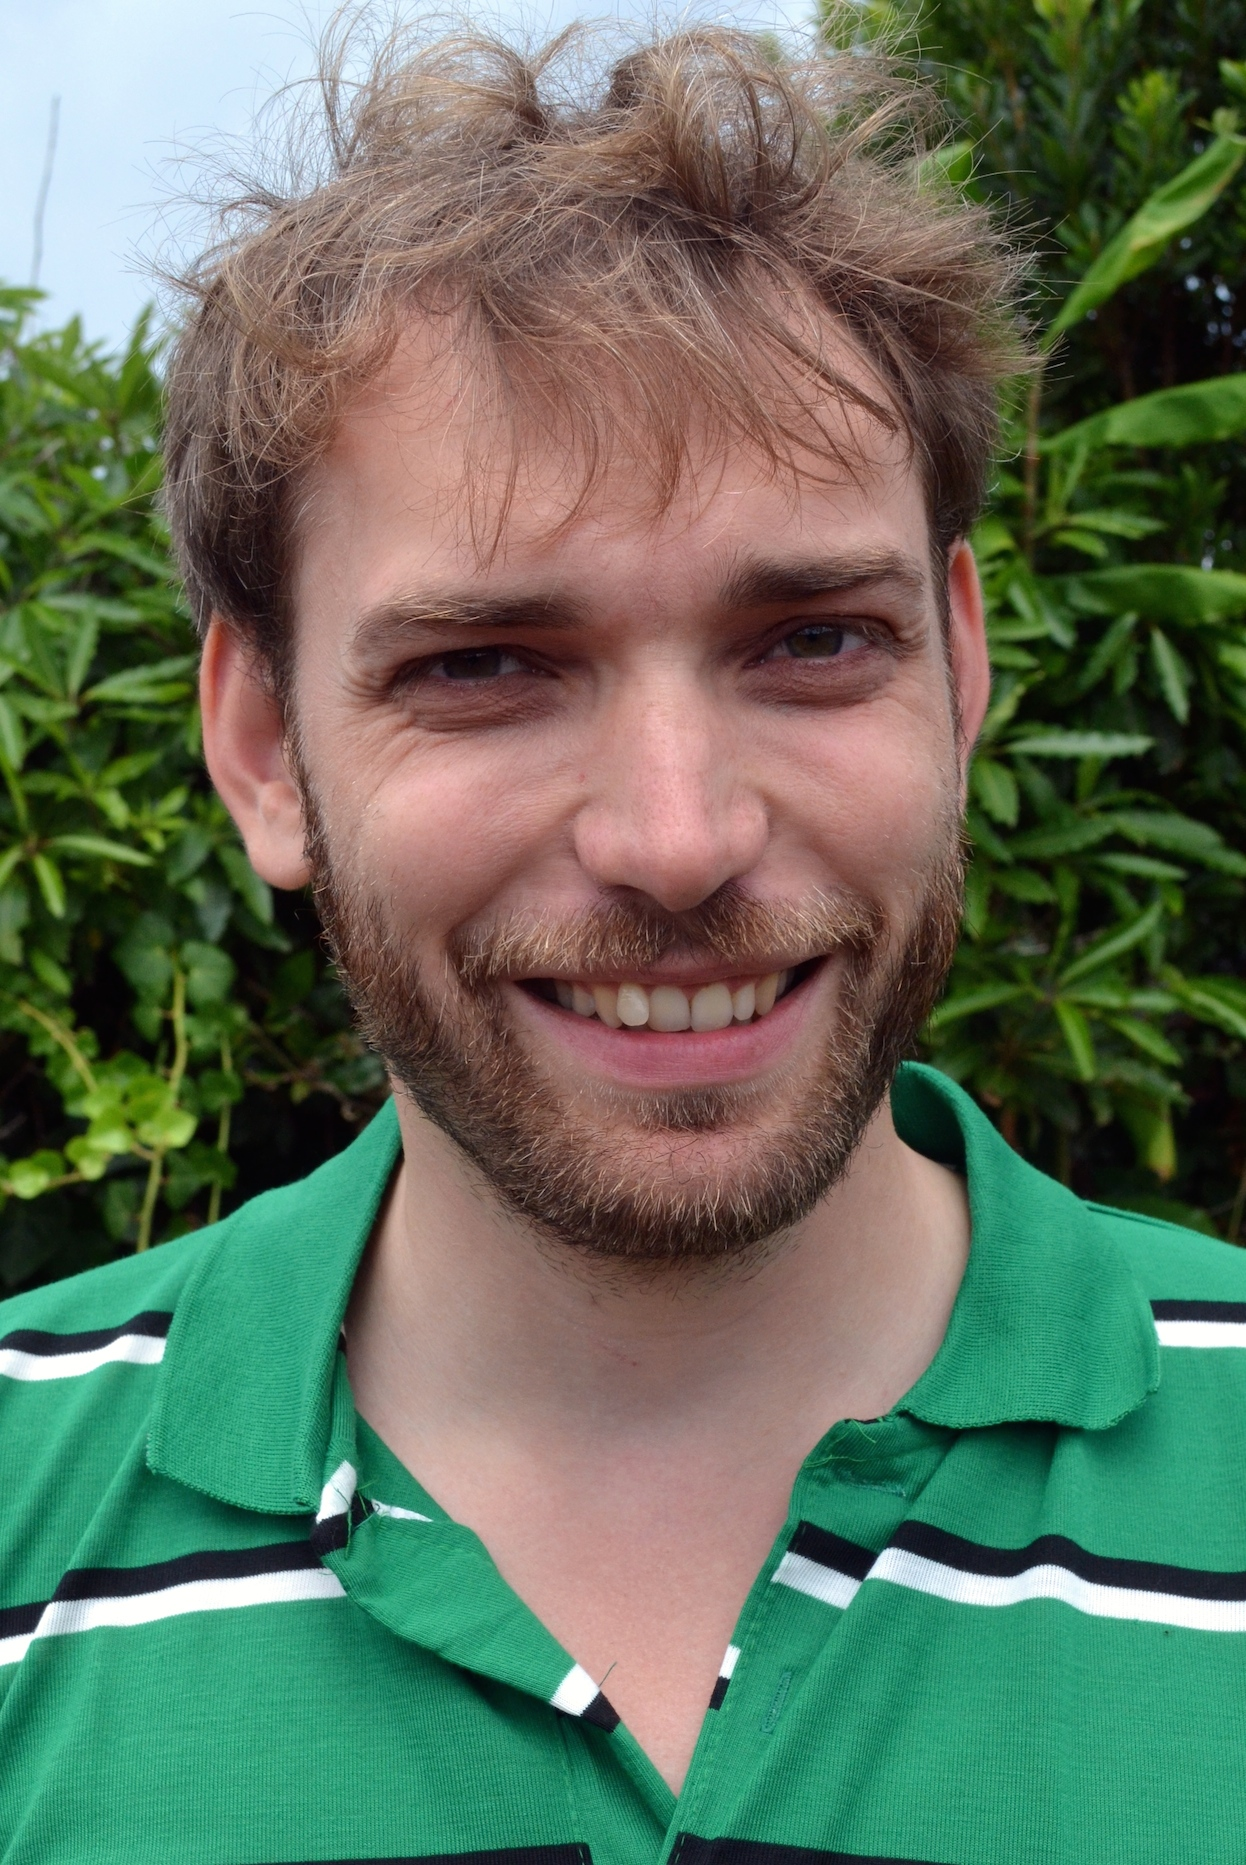
\includegraphics[height=10cm]{portrait}
\end{minipage}
% }}}

\vspace{-1cm}
\section*{Introduction}
{
\LARGE
We have previously reported the stability of the codon--anticodon interface
during mouse development, where we measured the whole-transcriptome codon
usage and the tRNA anticodon abundance of matching stages of development and
found remarkable stability, both in codon usage and in tRNA anticodon
abundance, despite the drastic phenotypic changes \citep{Schmitt:2014}.
These findings let us to hypothesise that, unlike in other organisms
\citep{Carlini:2003}, no widespread translational regulation, mediated by codon
bias, is likely to occur in mammals.\\
In contrast, others have recently reported that codon usage for genes
enriched in cell-autonomous function and multicelluarity in humans is
adapted to the tRNA abundance of proliferating and differentiating cells,
respectively \citep{Gingold:2014}.\\
Here we test this hypothesis using whole-genome expression data from healthy
liver tissue and two different tumour cell lines in human and mouse.
}

\vspace{-0.5cm}
\section*{Experimental setup}
\vspace{-0.5cm}
\begin{minipage}{0.15\textwidth}
    \centering
    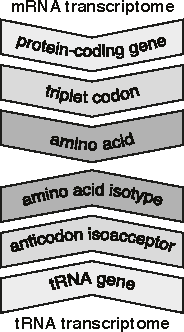
\includegraphics[height=17cm]{interaction-schema}
\end{minipage}%
\hfill
\begin{minipage}[t][][t]{0.50\textwidth}
    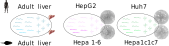
\includegraphics[width=\textwidth]{experimental-design}
    \\[0.5cm]
    Codon usage and anticodon abundance of healthy adult liver and two
    cancer cell lines were correlated to estimate their adaptation in each
    cellular condition. Higher correlation implies better adaptation of the
    codon usage to the anticodon abundance.

    The GO terms used for cell-specific functions are “pattern specification
    process” and “M phase of mitotic cell cycle” for healthy and tumour
    cells, respectively \citep{Gingold:2014}.
\end{minipage}%
\hfill
\begin{minipage}{0.23\textwidth}
    \centering
    \textbf{Legend:}\\[0.5cm]
    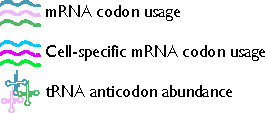
\includegraphics[width=\textwidth]{legend-1}
    \\[2cm]
    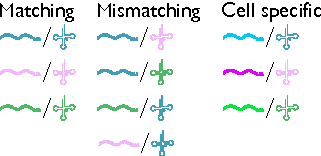
\includegraphics[width=\textwidth]{legend-2}
\end{minipage}%

\vspace{1cm}
\noindent
\begin{minipage}[t][][t]{0.48\textwidth}
    \section*{Codon usage bias correlates with gene set size}
    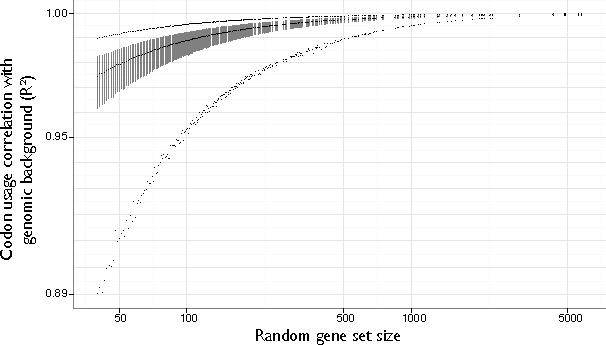
\includegraphics[width=\textwidth]{gene-set-size}
\end{minipage}%
\hfill
\begin{minipage}[t][][t]{0.48\textwidth}
    \section*{No evidence of codon--anticodon adaptation}
    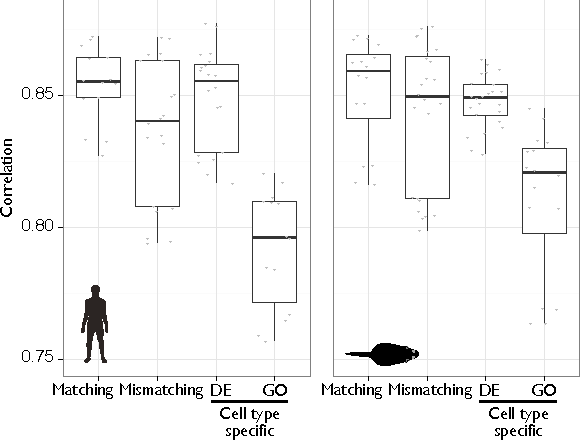
\includegraphics[width=\textwidth]{results}
\end{minipage}%

\vspace{-0.5cm}
\section*{Conclusion}
{
    \LARGE
    Codon--anticodon correlation is not significantly higher in matching
    than in mismatching cellular condition. The same is true in genes in
    condition-specific gene sets (determined either via \textbf Differential
    \textbf Expression or \textbf Gene \textbf Ontology). Gene sets determined from Gene Ontology,
    on the contrary, show significantly less codon--anticodon correlation,
    consistent with the stochastic effect of small gene set sample sizes
    (\(N<100\) in all cases) on codon bias.

    \hfill Contact: \textbf{rudolph@ebi.ac.uk}, \textbf{@klmr}
}

\vspace{-1cm}
\section*{References}
\vspace{-1.5cm}
\begin{multicols}{2}
    \renewcommand\section[2]{}
    \bibliography{references.bib}
\end{multicols}

\vfill
\noindent
\begin{center}
\normalsize%
1. European Molecular Biology Laboratory, European Bioinformatics Institute •
2. University of Cambridge, Cancer Research UK Cambridge Institute
\end{center}
\vspace{1cm}

\noindent
\begin{minipage}[][][b]{0.3\textwidth}
    \centering
    \includegraphics[height=4cm]{Colour_logo_pantone_DM}
\end{minipage}%
\hfill%
\begin{minipage}[][][b]{0.3\textwidth}
    \centering
    
\includegraphics[height=4cm]{cruk-logo}
\end{minipage}%
\hfill%
\begin{minipage}[][][b]{0.3\textwidth}
    \centering
    \includegraphics[height=4cm]{EMBL-EBIlogo}
\end{minipage}%
\end{document}
